% ILP (for ICCD'05)
%
%\documentclass[10pt,dvips]{article}
%\documentclass[10pt,dvips]{article}
\documentclass[10pt,twocolumn,dvips]{article}
\usepackage[english]{babel}
\usepackage{epsfig}
%\usepackage{fancyheadings}
%\usepackage[T1]{fontenc}
%\usepackage[latin1]{inputenc}
%\usepackage{twocolumn}
%\usepackage{verbatim,moreverb,doublespace}
%\usepackage{rotate,lscape,dcolumn,array,rotating,latexsym}
%
%\input{epsf}
%
% for (IEEE single-column format)
%\textwidth 6.875in
%\textheight 8.875in
%\topmargin -0.6in
%\oddsidemargin 0mm
%\evensidemargin 0mm
%
% for HPCA (IEEE two-column format)
%\textwidth 6.5in
%\textheight 8.875in
%\topmargin -0.4in
%\oddsidemargin 0mm
%\evensidemargin 0mm
%
% for ICCD'05
\textwidth 6.5in
\textheight 8.875in
\topmargin -0.4in
\oddsidemargin 0mm
\evensidemargin 0mm
%
%
% turn the following (linespread) on to 1.6 for "double space"
%\linespread{1.6}
%
%
% some publishers want no page numbers for final print
%\pagestyle{empty}
%
\begin{document}
%
%
\title{Unfinished Business: Extracting More Instruction Level Parallelism}
%
%
\author{
undisclosed
}
%
%
% some publishers do not want a data in the final print
\date{13th May 2005}
%
\maketitle
%
% uncomment the following for first page with no page number (for IEEE)
%\thispagestyle{empty}
%
%
\begin{abstract}
%
We present a new microarchitectural approach
for managing parallel and speculative instruction execution
within the processor.  
Instructions are allowed to enter into
execution without first determining control or data dependencies,
rather dependencies are 
determined dynamically at execution time.
This approach might be
characterized by first letting all instructions enter
into execution as there are available machine resources,
and then re-execute instructions as necessary in order
to converge on the correct program state for commitment.
Instructions are re-executed without being refetched or redispatched
(but re-issued)
as the correct input
dependencies are dynamically determined.
%
\end{abstract}
%
%
\vspace{-0.15in}
%\vspace{-0.25in}
\section{Introduction}
%\vspace{-0.15in}
%
Although many high performance applications today
can be parallelized at the application level 
and executed on tiled or clustered systems,
there are and will continue
to be requirements for achieving the highest performance
on single threaded highly serially dependent program codes.
We attempt to target this application problem space
through the extraction of instruction level parallelism (ILP).
The prospect of unprecedented numbers of transistors 
available in silicon (perhaps eventually approaching 10 billion
and beyond) represents an opportunity to capitalize on
the remaining ILP latent in even sequential (stubbornly non-parallizable)
programs.
With limits to performance improvement through clock cycle reduction
alone (witness also the recent flattening of higher clock frequencies),
methods such as more aggressive ILP extraction in the microarchitecture
become even more attractive.

Several studies into the limits of instruction level 
parallelism have shown that there is 
a significant amount of parallelism within
typical sequentially oriented single-threaded programs
(e.g., SpecInt-2000).  
The work of researchers including 
Lam and Wilson~\cite{Lam92},
Uht and Sindagi~\cite{Uht95},
Gonzalez and Gonzalez~\cite{Gon97}
have shown that there exists a great amount of instruction level
parallelism that is not being exploited by any existing
computer designs.
Generally, ILP extraction is achieved by introducing multiple
execution units into the microarchitecture and allowing each unit
to operate as independently and as parallel as possible, yielding
increased instructions per clock (IPC).
Maintaining binary compatibility with existing instruction
set architectures (ISA) is generally a requirement, so we
target this as well with our proposal.

Microarchitectures such as RAW~\cite{waingold97,taylor02}
or conventional cluster-based systems
address the issue of parallelism within applications but only do so
by exposing the spatially separated nature of their
parallel-processor systems to the compiler and the application itself.
This approach towards parallelism is an important one but
can only address those applications that can be parallelized at
a fairly course level.

Other microarchitectures that have employed the
use of multiple execution units for ILP extraction are the Multiscalar-like
processors~\cite{Sohi95,sundararaman97multiscalar},
the SuperThreaded processor model~\cite{tsai96superthread},
and
the Parallel Execution Window processor model~\cite{kemp96pew}.
The proposed MultiCluster machine model by 
Farkas et al.~\cite{farkas97multicluster} are also in this category.
Nagarajan also proposed a {\em Grid Architecture} of ALUs
connected by an operand network~\cite{Nag01}.  
However, unlike our work, all of these proposals have either
not achieved their performance objectives or have been found
difficult to implement, and have also generally relied on the
coordinated use of a the compiler along with a new ISA.

Our goal is a microarchitecture
that features the benefits of speculatively executing with 
relaxed control and data dependencies,
such as done in the proposed Superspeculative 
microarchitecture ~\cite{Lip97}, but with the ability
to managing a large number of instructions simultaneously in flight.
This makes the microarchitecture
suitable for programs normally constrained by short dependency chains.
An important distinction between our proposed microarchitecture and
that of most others is that we dispatch instructions to special structures
resembling reservation stations~\cite{Anderson67,Tom67},
but instead of the instruction
vacating the station upon instruction issue, it
remains in the station until retirement.
Instructions also
dynamically determine their proper input dependencies,
executing and re-executing as needed as new dependencies
are determined.

The rest of this paper is organized as follows.
Section 2 gives an overview of the microarchitecture.
Section 3 provides some further details on the more
novel and core components of the microarchitecture.
Section 4 provides some characterization and performance 
results for our microarchitecture through the simulated
execution of benchmark programs.
We summarize in Section 5.
%
\vspace{-0.15in}
%\vspace{-0.25in}
\section{Microarchitecture overview}
%\vspace{-0.15in}
%
The handling of main memory, and the cache hierarchy 
through the L1 instruction and L1 data caches are all
conventional and similar to existing microarchitectures.
Instruction fetch is also rather conventional.
We also employ: a
load-store-queue (LSQ) component, an architected register file,
structures that closely resemble reservation stations or issue
window slots, and rather conventional execution function units.

The most novel aspect of our microarchitecture is how we
handle instruction issue for execution and re-execution.
In order to efficiently handle instruction issue and re-issue,
we employ a structure somewhat similar to
a reservation station but with additional state and control
logic.  
This new structure is termed
an \textit{issue station} (IS).
Like other machines with reservation stations, we dispatch 
decoded instructions from the fetch unit to these issue stations
when one or more of them are empty (available for dispatch) or 
becoming empty on the next clock cycle.  
Instructions are dispatched in-order.
The number of instructions dispatched in any 
given clock cycle is
the lesser of the number of issue stations available and the
dispatch width (as counted in numbers of instructions).
Instructions are always dispatched to issue stations when
some are free (or becoming free) and are generally dispatched
without first knowing their input dependencies or having those
corresponding operands available.
Rather, all operand dependencies are determined dynamically through
snooping after instruction dispatch.

Once instructions are dispatched to issue stations,
they wait for plausible (generally speculative) input operands
to be snarfed and then
contend for execution resources if necessary for the execution
of the instruction.
Results of instruction executions are retained within
the issue station until retirement.  
Forwarding of instruction execution
results is done from the issue station itself, rather from the
FU (if one was used).
This arrangement allows for some simple instructions to be executed within
the issue without circulating through the function unit
pipelines.  
Since an issue station is allocated for an instruction for
its lifetime, this represents a ready resource and place for simple
instructions to execute, for those instructions that do 
not require substantial execution logic.  
This situation is employed to minimally execute all
control-flow and load-store instructions within the
issue station itself.
Remaining instructions contend for 
function unit availability for their executions.
The process of winning a function unit execution-slot constitutes
an instruction issue, and is entirely out of order (as with
all other executions).

Instruction commitment can occur on each clock, is in-order, and
proceeds from the oldest program-ordered
instruction through younger instructions until an instruction
is reached that doesn't meet the requirements for commitment.
Instructions can only commit if they have executed at least once,
are not in the process of receiving updated inputs (which could
trigger re-execution and a different committed result),
and are finished forwarding output operands 
to younger program-ordered instructions.  
The last constraint guarantees that all younger
instructions can process the final output operands of older
instructions.
Since the process of forwarding output operands can take several
clocks due to forwarding bandwidth constraints, this can be
an additional source of delaying commitment.

Figure \ref{fig:overview} shows a high-level block diagram
of our microarchitecture showing the major instruction execution components.
The memory hierarchy, as well as details of the instruction fetch
unit, are not shown as they are similar to those of existing
machines.
%
\begin{figure}
\scriptsize {
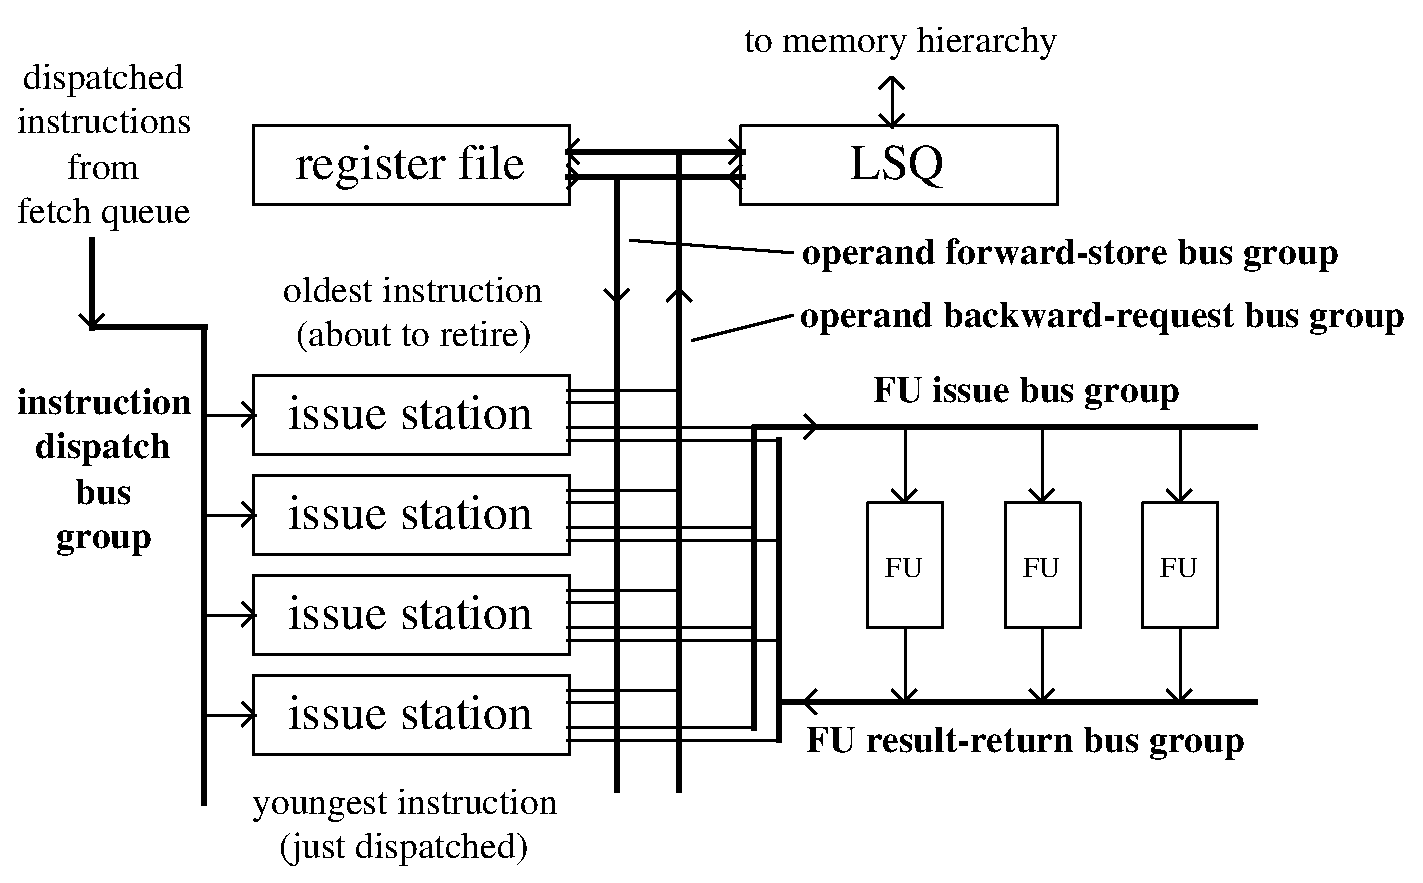
\epsfig{file=figure1.eps,width=3.0in}
}
\caption{{\em High-level block diagram of our microarchitecture.} 
Issues stations are shown on the left and various function
units on the right.  An architected register file and a
load-store-queue is shown at the top.
Bidirectional operand request and forwarding buses are shown
vertically oriented (to the right of the Issue Stations).
Buses to transport an instruction operation and its source operands
to the function units are also shown. 
Likewise buses to return result operands are present.}
\label{fig:overview}
\end{figure}
%
There is only one load-store-queue (LSQ) and
architected register file (containing only
committed registers) but the numbers of all other components can
vary with a specific machine implementation.
All issue stations are identical, allowing for any
instruction to be dispatched to each.
Function units can be duplicated and functional differentiated
as desired. 

Buses are provided (shown mostly horizontally in the figure)
for bringing instruction codes and operands from the issue
stations to the FUs and back again.
The number of parallel buses provided in each bus group is
an implementation option.
The vertical buses, roughly in the center of the figure
labeled \textit{operand forward-store} and
\textit{operand backward-request}, are
bidirectional and multi-master bus groups that
allow for operands to be requested from and forwarded to
issue stations.
This is the means by which instruction acquire their necessary
operands for proper execution.
Operand requests also to the register file and LSQ, and they
can likewise forward operands in response to requests.
All buses are statistically multiplexed, although other
arrangements are certainly also possible.

Collectively, all of the components discussed in this section
(and shown in 
Figure \ref{fig:overview}) are termed the \textit{execution window}.
Although the minimum of the number of FUs and the buses to them
corresponds to the issue width in more conventional machines,
the effective IPC of the machine can exceed this number since
some instructions
execute entirely within the issue stations.
%
\vspace{-0.15in}
%\vspace{-0.25in}
\section{Core component detail}
%\vspace{-0.15in}
%
%\vspace{-0.25in}
\subsection{Issue Stations}
%\vspace{-0.15in}
%
The issue stations provide the most significant distinction of this
microarchitecture from most others.  
These are similar to reservation stations
but contain additional state and logic that allows
for dynamic operand dependency determination as well as
for holding a dispatched instruction (its decoded form) 
until it is ready to be retired.  
There is state inside the station that is relevant to
the instruction itself and specific
to the operands of that instruction (both source and
destination operands).

The state that is primarily associated with the instruction itself
consists of :
%
\begin{itemize}
\vspace{-0.10in}
\item{instruction address}
\vspace{-0.10in}
\item{instruction operation}
\vspace{-0.10in}
\item{execution state}
\vspace{-0.10in}
\item{time ordering tag}
\vspace{-0.10in}
\item{instruction predication information}
\vspace{-0.10in}
\end{itemize}   
%
The \textit{instruction operation} is derived from the decoded
instruction and specifies the instruction class and other
details needed for the execution of the instruction.
This information may consist of subfields and is generally ISA
specific.
The \textit{instruction address} and \textit{predicate} state
are only used when dynamic predication~\cite{undisclosed2}
is done within the microarchitecture.
The \textit{time tag} value is used to order this instruction
with respect to all others that are currently within the execution
window of the machine.
The time tag is also used as part of the operand snooping
logic (discussed more later).
It is a small positive integer, large enough to represent
the number of issue stations in a particular implementation.
The \textit{execution state} value constitutes the state
used by various state machines within the issue station
for controlling its operation and for determining readiness
for commitment.

The remainder of the state consists of one or more input
source operands and one or more output destination operands.
All operands regardless of type and whether source or destination
occupy a similar structure within an issue station, termed an
\textit{operand block}.
More detail on these operand blocks and operand management
is provided in the next section.

A simplified block diagram of our issue station is shown in 
Figure \ref{fig:issuestation}.
%
\begin{figure}
\scriptsize {
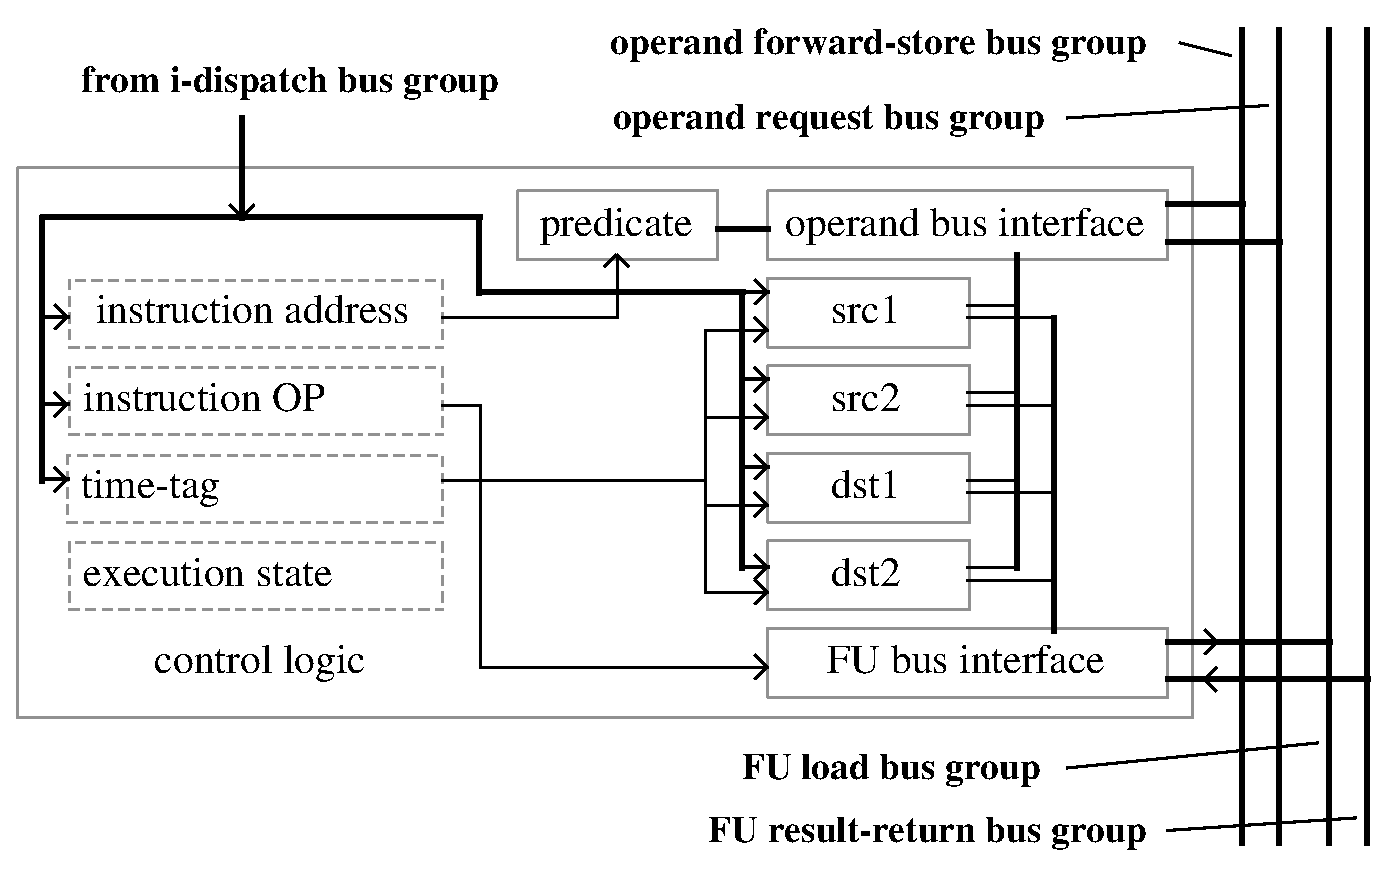
\epsfig{file=figure2.eps,width=3.0in}
}
\caption{{\em High-level block diagram of our Issue Station.} 
The major state and sub-blocks associated with an Issue Station is shown.
General instruction state (shown in dash-lined boxes) is
on the left, while
four operand blocks (two source and two destination),
and the four primary bus group interfaces (grouped by function at
upper right and lower right) to the rest of the
execution window are on the right.}
\label{fig:issuestation}
\end{figure}
%
In this example, a total of four operand blocks are shown, labeled:
\textit{src1}, 
\textit{src2}, 
\textit{dst1}, 
and \textit{dst2}.
The number of source and destination operand blocks that are
used for any given machine is dependent upon the requirements
of the ISA implemented.
%
%
%\vspace{-0.25in}
\subsection{Operands}
%\vspace{-0.15in}
%
The types of operands are distinguished: register and memory.
Operands blocks are constructed to hold either type.
The state within an operand block consists of :
%
\begin{itemize}
\vspace{-0.10in}
\item{type of operand}
\vspace{-0.10in}
\item{time ordering tag}
\vspace{-0.10in}
\item{address}
\vspace{-0.10in}
\item{size}
\vspace{-0.10in}
\item{previous value}
\vspace{-0.10in}
\item{value}
\vspace{-0.10in}
\end{itemize}   
%
The operand \textit{time ordering tag}
serves
an analogous purpose as the time-tag register within an issue station,
except that it applies specifically to this particular
operand rather than to the instruction as a whole.
Again, this time tag is used in the operand snooping logic
and allowed for the dynamic discovery of dependencies
for instructions.

The \textit{address} field differs
depending on the type of the operand.
For register operands, the address would be
the name of the architected register.
All ISA architected registers are typically provided a
unique numerical address.  These would include the
general purpose registers, any status or other non-general
purpose registers, and any possible ISA (architected) predicate registers
(like those in the iA-64 ISA~\cite{intel99ia,schlansker00epic}.
For memory operands, the identifying address is just the
programmer-visible architected memory address of the corresponding
memory value.

The \textit{size} is only used for memory operands and holds
its size in bytes.
The \textit{value} holds the present value of the operand
calculated from this present instruction (if it has executed
at least once).
The \textit{previous value} is only used for destination
operands and holds the value that the operand
had before it may have been changed by the execution of 
the present instruction.
The previous value is used 
when a forwarded operand with a specific
address was incorrect.
This situation occurs when addresses for memory operands are
speculatively calculated but are later determined to have changed.
An operand with the old address is forwarded with the previous
value to correct the situation.

Figure \ref{fig:operand} shows a simplified block diagram of
an operand block along with its major data paths for its
primary functions: snoop-snarf, operand-forward, FU-issue,
and FU-store-result.
%
\begin{figure}
\scriptsize {
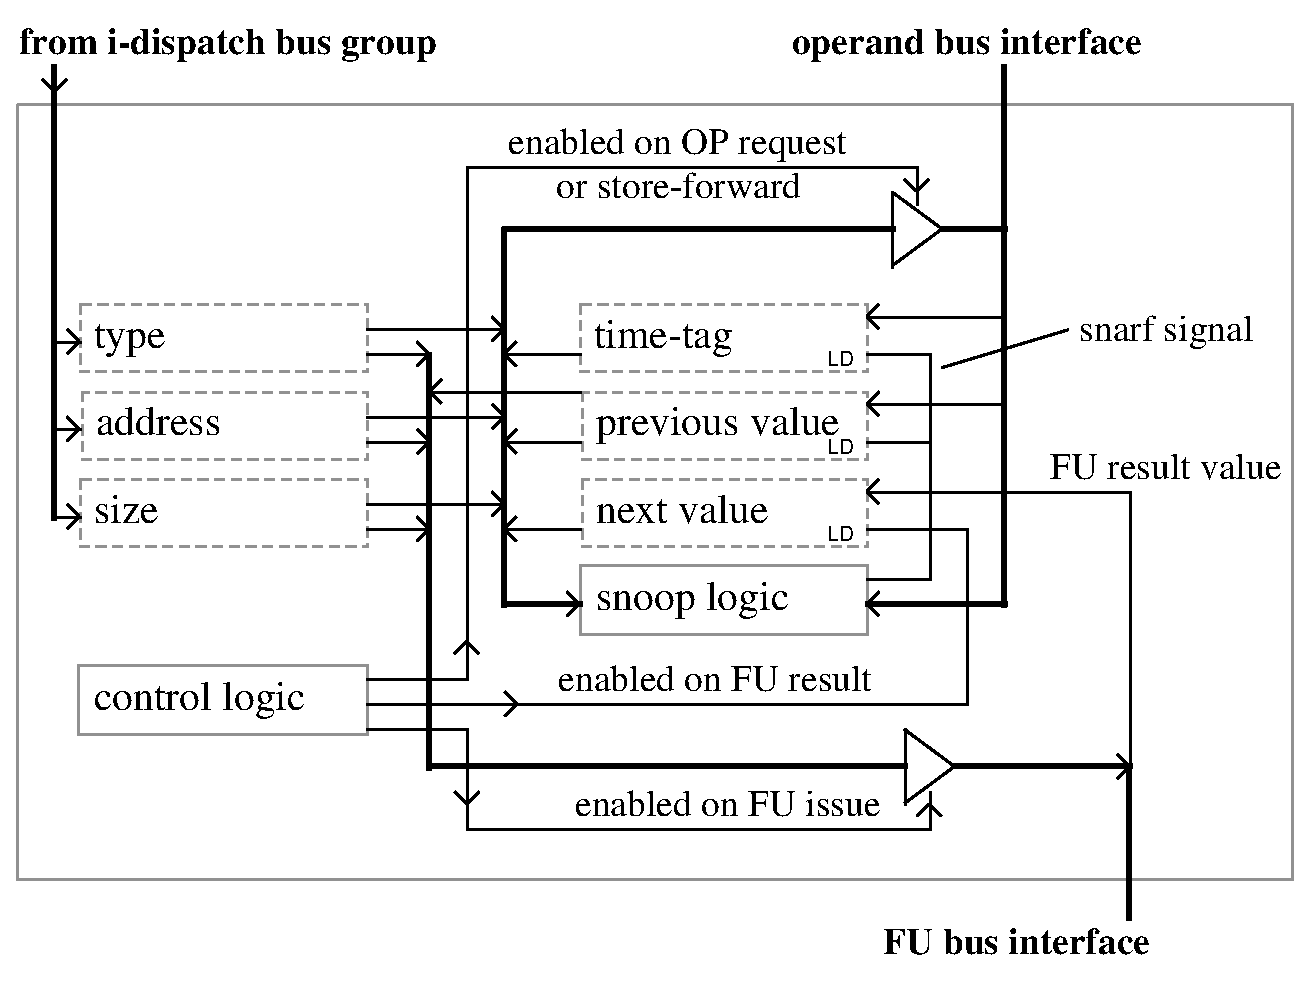
\epsfig{file=figure3.eps,width=3.0in}
}
\caption{{\em Block diagram of an Operand Block.} 
Each Operand Block holds an effectively renamed 
operand within the Issue Stations.
Several operand blocks are employed within each Issue Station
depending on the needs of the ISA being implemented.
The primary state register information maintained for each operand (shown in
dash-lined boxes)
along with the major data paths and enabling signals for
its major functions are shown.}
\label{fig:operand}
\end{figure}
%

In effect, a full renaming of
all operands is realized for all instructions
in flight in the machine.  
All false dependencies are thusly avoided.
Operand names consist of the components :
%
\begin{itemize}
\vspace{-0.10in}
\item{type of operand}
\vspace{-0.10in}
\item{time tag}
\vspace{-0.10in}
\item{address}
\vspace{-0.10in}
\end{itemize}   
%
%
%
%\vspace{-0.25in}
\subsection{Operand forwarding and snooping}
%\vspace{-0.15in}
%
Operands resulting from the execution of instructions
are transmitted forward (on the forwarding bus fabric)
or use by younger (in program order) waiting instructions.
All forwarded operands are snooped by operand blocks
contained within those issue stations containing younger
dispatched instructions.
The information associated with each operand that is
forwarded is referred
to as a {\em transaction} and consists of :
%
\begin{itemize}
\vspace{-0.10in}
\item{transaction type}
\vspace{-0.10in}
\item{operand type}
\vspace{-0.10in}
\item{address}
\vspace{-0.10in}
\item{time tag of the originating issue station}
\vspace{-0.10in}
\item{data value for this operand}
\vspace{-0.10in}
\end{itemize}   
%
The time-tag forwarded with the operand is that of the originating
issue station (instruction instance).
The operand information above is typical of both
register and memory operand transactions and the use
of the \textit{operand type} distinguishes one from the other.
The \textit{transaction type} field is used to 
designate whether the transaction represents a store from
a previous instruction or an indications that
a previously forwarded operand is no longer valid.
A number of management mechanisms are possible but
these are beyond the scope of this present work.

A snarf for a particular operand
within an issue station occurs when: the operand type and address
of the snooped operand match that of the stored operand, and
the snooped time-tag is both less than the current instruction
time-tag (stored in the issue station) and is less than or
equal to the last time-tag snarfed for the given stored operand.
In the case of a snarf, the stored operand time-tag (TT) and
previous-value (PV) registers are reloaded with the associated
fields from the snooped operand transaction.
Additionally, if the snooped operand data value is different
than the stored operand previous-value, an execution or a re-execution
is scheduled for the current issue station.
However, if the snooped data value equals the stored
data previous-value, no new execution is triggered.
This eliminates unnecessary re-execution for silent register updates
from previous (program-ordered past) instructions.

A simplified schematic diagram of the logic used for operand snooping
is shown in Figure \ref{fig:source}.
The {\em time-tag} and
{\em previous-value} registers within an operand block
are reloaded with new values on each snarf,
while the
{\em instruction time-tag} register in the issue station
is only loaded when an instruction is dispatched.
The operand block {\em address} register is either loaded at instruction
dispatch or may be loaded during instruction execution for some
instructions
(for example by load/store instructions).
%
\begin{figure}
\scriptsize {
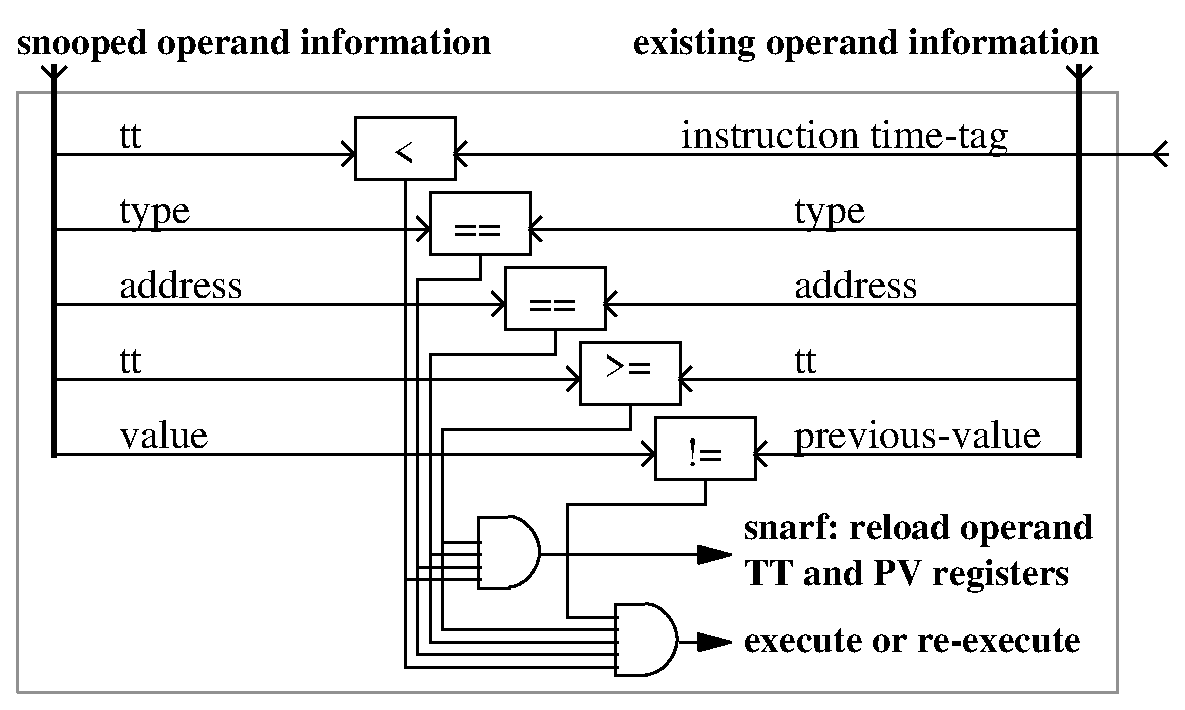
\epsfig{file=figure4.eps,width=3.0in}
}
\caption{{\em Snooping logic for operand updates.} 
The snooping
logic for one of several possible source operands is shown.
This logic would reside in each of the operand blocks within an 
issue station and they would all perform the snoop operation
simultaneously.
Just one operand forwarding bus is shown being snooped but
typically several forwarding buses are snooped simultaneously.}
\label{fig:source}
\end{figure}
%
%
\vspace{-0.15in}
%\vspace{-0.25in}
\section{Experimental results}
%\vspace{-0.15in}
%
In this section we present a first look at some
experimental results from simulation
of the machine presented.
We use ten of Spec2000 integer benchmarks 
(listed in Table ~\ref{tab:results} below) to evaluate the potential
of this microarchitecture. 
For all simulations, the initialization phases of all
programs are skipped using a fast-forward mechanism.
This allows the subsequent functional simulation (which takes
the real bulk of simulation time) to operate on the most
characteristic part of the benchmarks.
After the initial fast-forward operation, a phase of one million 
instructions are executed in such
a way as to warm up machine components that have longer
state residency times.  This currently includes the cache hierarchy
(L1 and L2 caches) and the branch predictor.
Then a short sequence of instructions are 
executed to prime machine components such as the issue stations.
This sequence is approximately equal to two times the number
of issues stations configured for the target machine.
Finally, we execute on the main functional cycle simulator
for the next 100 million instructions.  

For all simulations, we used separate instruction and
data L1 caches, but a unified L2 cache.
The data caches use a write-back policy with a least recently used
block replacement algorithm.
The execution window is flushed of younger (speculative) instructions
on a branch misprediction (the same as most conventional machines).
Other configuration parameters of the machine for the
simulations are shown in Table~\ref{tab:baseline}.

%
\begin{table}
\begin{center}
\caption{{\em General machine characteristics.}
These machine parameters are used for all simulations
unless otherwise specified.}
\label{tab:baseline}
\scriptsize{
\begin{tabular}{|l|l|}
\hline 
L1 I cache access latency&1 clock\\
\hline
L1 I cache size&32 KBytes\\
\hline
L1 I block size&32 bytes\\
\hline
L1 I organization&direct mapped\\
%
\hline 
L1 D cache access latency&2 clocks\\
\hline
L1 D cache size&128 KBytes\\
\hline
L1 D block size&32 bytes\\
\hline
L1 D organization&2-way set assoc.\\
%
\hline
L2 cache access latency&20 clocks\\
\hline
L2 cache size&1 MBytes\\
\hline
L2 block size&32 bytes\\
\hline
L2 organization&4-way set assoc.\\
%
\hline
main memory access latency&150 clocks\\
\hline
branch predictor&2-level w/ XOR\\
\cline{2-2}
 & 16k PHT entries\\
\cline{2-2}
 & 8 history bits\\
\cline{2-2}
 & 32k BHT entries\\
\cline{2-2}
 & sat. 2-bit counter\\
\hline
fetch width & 8 instructions \\
\hline
FU issue width & 4 operations \\
\hline
issue width & 4 \\
\hline
number integer FUs & 4 \\
\hline
number other FUs & 1 each \\
\hline
forwarding buses & 8 \\
\hline
bus traversal latency & 1 clock \\
\hline
integer FU latency & 1 clock \\
\hline
other FU latencies & 3 to 17 clocks \\
\hline 
\end{tabular}
}
\end{center}
\end{table}
%

We present the IPC results of our proposed
microarchitecture with that of a baseline 
superscalar microarchitecture that is similarly configured.
We used the 
Simplescalar MASE framework~\cite{Austin97}
to simulate a conventional superscalar (approximately a MIPS R10000
in the case of SimpleScalar MASE).

The baseline superscalar machine includes an instruction
window consisting of reservation stations and a re-order buffer (ROB)
to store speculative execution result registers pending commitment.
Instructions for the baseline superscalar are fetched and dispatched
to the instruction window where they wait for input data dependencies to
become ready.  When all instruction input dependencies are ready,
and as issue bandwidth allows, instructions are issued to the
function-unit pipelines.  Register results are stored in the ROB
until commitment.  
Both the baseline superscalar and our proposed
microarchitecture flush the execution window on a resolved mispredicted 
conditional branch.
This is a fairly typical superscalar execution
arrangement and is fixed in the Simplescalar MASE simulator.

Although an exact comparison of the two machines is not possible
due to their very different construction, we have arranged
for both the baseline machine and our proposal to have either an
exact or a very
close correspondence in the amount and number of hardware resources.
Both machines are configured with identical
cache arrangements and cache configurations.
Both also employ the same branch predictor and predictor configuration.
Both also implement a four-wide issue machine.
For both machines, the issue width is the maximum number of
instructions that can be issued in a single clock cycle.
However the baseline superscalar employs reservation stations and
an ROB while our microarchitecture uses our novel issue stations.
We therefore roughly equate the number of issue stations of
the proposed machine with the combination of both the
number of instruction window slots (reservation stations)
and ROB entries of the baseline superscalar.
Our results are for 128 issues stations in the proposed 
microarchitecture and both 128 issue window slots (reservation stations)
and 128 ROB entries for the baseline superscalar.
This represents a modest sized machine of today.

The IPC results for the baseline superscalar and our proposed
machine are shown in columns two and three of Table~\ref{tab:results}
respectively.
Column 4 (labeled REX) gives the percent additional instructions
executed as compared with the number of committed 
instructions.
We also calculated the harmonic mean of the IPC
across all benchmarks.
Columns 5 and 6 are described later.
%
\begin{table}[p]
\begin{center}
\caption{{\em IPC and re-execution results.}
IPC performance of a MASE baseline superscalar machine and our
proposed microarchitecture is presented.
The column titled REX gives the percent of 
extra instructions executed for the proposed machine as compared with 
the committed instructions.}
\label{tab:results}
\vspace{+0.1in}
\scriptsize {
\begin{tabular}{|l||r|r|r|r|r|}
\hline
 & baseline &
 \multicolumn{2}{c|}{proposed} &
 \multicolumn{2}{c|}{proposed-extra} \\
\cline{2-6}
 & IPC & IPC & REX & IPC & REX \\

\hline
bzip2&
2.1 & 1.98 & 97.8\% & 2.41 & 86.1\% \\

\hline
crafty&
1.3 & 1.96 & 79.2\% & 2.33 & 90.9\% \\

\hline
eon&
1.3 & 2.62 & 110.4\% & 3.12 & 91.7\% \\

\hline
gcc&
1.3 & 1.70 & 96.2\% & 2.41 & 45.5\% \\

\hline
gzip&
1.4 & 1.42 & 98.0\% & 1.93 & 94.3\% \\

\hline
parser&
0.8 & 1.23 & 115.8\% & 1.41 & 100.2\% \\

\hline
perlbmk&
0.6 & 1.44 & 92.3\% & 1.52 & 55.3\% \\

\hline
twolf&
1.2 & 1.32 & 88.2\% & 1.60 & 78.9\% \\

\hline
vortex&
1.0 & 2.61 & 103.7\% & 3.75 & 40.3\% \\

\hline
vpr&
1.0 & 1.13 & 96.1\% & 1.39 & 72.0\% \\

\hline
H-MEAN&
1.1 & 1.61 & & 1.97 & \\

\hline
\end{tabular}
}
\end{center}
\end{table}
%
As can be seen, our proposed machine attains a speedup of approximately
1.46 (46\% better) as compared with the baseline superscalar 
(comparing columns two and three) 
while using approximately the same amount of hardware resources.
Column four of Table~\ref{tab:results} (titled REX) shows the percentage
of committed instructions that incurred re-executions.
Most benchmarks exhibit a behavior of executing somewhere around
200\% (within about plus or minus 20\%) of the committed
number of instructions.
This compares similarly to the amount of execution needed
in proposals like the SlipStream processor~\cite{ibrahim03},
except that neither two threads nor two processors need be
dedicated to the execution of a single program, as it done in
that processor. 
Rather, approximately two times the execution was performed
within the resources of a single core and threaded machine.

Column 5 provides the IPC results for a version of the
machine where additional instructions are executed within
the issue stations as compared with the machine of column 3.
Minimally, control-flow and memory load-store instructions
are executed in the issue stations.  
However with a very small additional amount of silicon,
simple bit-logic instructions and integer add and subtract
instructions (including integer compare) can also 
be executed within the issue stations.
This arrangement (transistors permitting) increases the
amount of resources available for executions, thus increasing
parallelism and IPC performance.
This yields approximately 22\% better IPC performance
than with the minimal configuration proposed machine, and approximately
79\% IPC improvement of the baseline machine.
Column 6 shows the extra executions (re-executions) for
this latter arrangement.
For all benchmarks except for BZIP2, the number of re-executions
falls, sometimes dramatically, as compared with the original
arrangement.
However, it should be noted that due to the unrestrained
behavior of the machine to dynamically determine dependencies
and acquire new input operands, there is no way clear way to predict how
the number of re-executions is affected by certain machine
configuration changes.
In general the number of re-executions is a function of
the random execution order of instructions and the amount of
time for them to convert on a committed set of outputs.
This behavior is the subject of further research.
%
%
\vspace{-0.15in}
%\vspace{-0.25in}
\section{Summary}
%\vspace{-0.15in}
%
We have described a new microarchitecture that
allows for both control and data speculative execution,
but also does so 
in a way where necessary re-executions are handled
quickly and cheaply in the hardware, without requiring either
re-fetch or re-dispatch.  
The necessary and complicated instruction dependency
enforcement is achieved dynamically during execution (and re-execution)
using time-ordering tags that maintain relative program order
of instructions and all operands in flight.
Binary program compatibility with existing ISAs (an important feature
in the market place) is also maintained with our proposal.
Our results show that our proposed machine achieves approximately
46\% better IPC performance over a conventional machine of roughly
equivalent silicon resources, and approximately a 79\%
IPC improvement given some modest additional silicon to facilitate
executing additional instructions in the issue stations.
Future work will explore the characteristics of even larger
sized machines with increased numbers of core components.
%
\bibliographystyle{latex8}
\bibliography{ilp}
%
\end{document}
%
%
%
